\documentclass{beamer}
\usepackage[utf8]{inputenc}
\usepackage{amsmath,amsfonts,amsthm,amstext,amssymb, xcolor, tikz, pgf}

% ----------------------------------------------------------
% Theme Setup

% Use Metropolis Theme
\usetheme[numbering=fraction]{metropolis}
\setbeamertemplate{blocks}[rounded][shadow=false]
\makeatletter
\setlength{\metropolis@titleseparator@linewidth}{1pt}
\makeatother



% Define Colors
\definecolor{chargerblue}{HTML}{002764}
\definecolor{chargerred}{HTML}{e02034}
\definecolor{bggray}{HTML}{d0d3d4}

% Set Colors
\setbeamercolor{title}{fg=chargerblue}
\setbeamercolor{background canvas}{bg=white}
\setbeamercolor{title separator}{fg=chargerred}
\setbeamercolor{structure}{fg=chargerblue}
\setbeamercolor{frametitle}{fg=white, bg=chargerblue}
\setbeamercolor*{normal text}{fg=chargerblue}
\setbeamercolor*{block body}{bg=white}
\setbeamercolor*{block title}{bg=chargerblue, fg=white}
% ----------------------------------------------------------

% ----------------------------------------------------------
% Custom Definitions, Commands, Environments, etc.

% Sets of numbers
\def\R{\mathbb{R}} % The reals
\def\N{\mathbb{N}} % The naturals
\def\Z{\mathbb{Z}} % The integers
\def\Q{\mathbb{Q}} % The rationals

% Blank space
\newcommand{\blank}[1]{\underline{\hspace{#1}}} % Blank space

% Fitted inclusion symbols
\newcommand{\fp}[1]{\left({#1}\right)} % Fitted parentheses around content
\newcommand{\fb}[1]{\left[{#1}\right]} % Fitted brackets
\newcommand{\set}[1]{\left\{{#1}\right\}} % Fitted braces (useful for sets)
\newcommand{\av}[1]{\left|{#1}\right|} % Fitted absolute value bars

% Coordinate Plane (Four-Quadrant)
\def\coordplane {
	\begin{tikzpicture}
		\draw[step=0.25cm,black,very thin,opacity=0.25] (-2.5cm, -2.5cm) grid (2.5cm, 2.5cm);
		\draw[<->,thick,black] (-2.5cm, 0) -- (2.5cm, 0) node[anchor=north west,pos=0.94,font=\scriptsize]{$x$};
		\draw[<->,thick,black] (0,-2.5cm) -- (0, 2.5cm) node[anchor=south east,font=\scriptsize,pos=0.94]{$y$};
	\end{tikzpicture}
}

% Coordinate Plane (One-Quadrant)
\def\onequad {
	\begin{tikzpicture}
		\draw[step=0.25cm, black, very thin, opacity=0.25] (0,0) grid (7.5cm,5cm);
		\draw[->, thick, black] (0,0) -- (7.5cm, 0) node[anchor=north west,font=\scriptsize,pos=0.94]{$x$};
		\draw[->, black, thick] (0,0) -- (0,5cm) node[anchor=south east,font=\scriptsize,pos=0.94]{$y$};
	\end{tikzpicture}
}
% ----------------------------------------------------------


% ----------------------------------------------------------
% Presentation Information 
\title[P.5 and P.6]{Rational Expressions; The Coordinate Plane}
\subtitle{Sections P.5 and P.6}
\author{Jacob Ayers}
\institute{MAT 130} % Course Name
\date{Lesson \#3} % Lesson #
% ----------------------------------------------------------

\begin{document}

% Slide 1 (Title Slide)
\begin{frame}
\titlepage
\end{frame}

% Slide 2 (Objectives)
\begin{frame}[t]{Objectives}
\begin{itemize}
	\item Find the domain of an algebraic expression
	\item Simplify rational expressions and complex fractions
	\item Add, subtract, multiply, and divide rational expressions
	\item Use the distance and midpoint formulas to solve applied problems
\end{itemize}
\end{frame}

\begin{frame}[t]{Domain}
The \textit{domain} of an algebraic expression is the set of real numbers for which it is defined. \vspace{6pt}

\pause

When finding domain, I recommend determining which values cannot be substituted into the function; the domain is everything else. \vspace{6pt}

\pause

There are two common situations when a number won't ``work" in an expression: \vspace{-4pt} \begin{enumerate}[1)]
\item When it results in a denominator of zero
\item When it results in taking an even-numbered root (e.g. square root) of a negative number
\end{enumerate}
\end{frame}

\begin{frame}[t]{Finding Domain}
Find the domain of the expression $3x^2 + 5x - 2$.

\pause \vfill

Find the domain of the expression $\sqrt{x+5}$.
\end{frame}

\begin{frame}[t]{Finding Domain}
Find the domain of the expression $\dfrac{3}{4x + 1}$

\pause \vfill

Find the domain of the expression $\dfrac{\sqrt{x-5}}{x-6}$
\end{frame}

\begin{frame}[t]{Simplifying Rational Expressions}
A \textit{rational expression} is a fraction in which the numerator and/or the denominator are polynomial expressions.

To simplify a rational expression, we factor each expression if possible and cancel common terms.

\pause

Simplify $\dfrac{x^3 + 64}{x^2 - 4x + 16}$
\end{frame}

\begin{frame}[t]{Simplifying Rational Expressions}
Simplify $\dfrac{4x+12}{x^2 - 3x - 18}$

\pause \vfill

Note that, when thinking about domain restrictions, we look at the \textit{original expression} rather than the simplified expression. In the original expression, the domain is $x \neq -3$, $x \neq 6$.

\end{frame}

\begin{frame}[t]{Operations with Rational Expressions}
Operations with rational expressions are identical to operations with fractions. First, factor all factorable expressions. \pause

To add or subtract rational expressions, a like denominator is needed before adding. \pause

To multiply rational expressions, multiply the numerators and multiply the denominators. \pause

To divide rational expressions, multiply by the reciprocal of the denominator.
\end{frame}

\begin{frame}[t]{Operations with Rational Expressions}
Simplify: $\dfrac{3}{x-1} - \dfrac{2}{x} + \dfrac{x+3}{x^2 - 1}$
\end{frame}

\begin{frame}[t]{Operations with Rational Expressions}
Simplify: $\dfrac{15x^2 + 5x}{x^3 - 3x^2 - 18x} \cdot \dfrac{x^2 - 2x - 15}{3x^2 - 8x - 3}$

\pause \vfill

Simplify: $\dfrac{x^3 - 1}{x^2 - 1} \div \dfrac{x^2 + x + 1}{x^2 + 2x + 1}$
\end{frame}

\begin{frame}[t]{Complex Fractions}
A \textit{complex fraction} is a fraction in which the numerator and/or denominator is a fraction.

Complex fractions look ugly, but they're really just fraction division.
\end{frame}

\begin{frame}[t]{Complex Fractions}
Simplify: $\dfrac{\frac{x + 3}{x - 4}}{\frac{x^2 - 8x + 16}{x^2 + x - 12}}$

\pause \vfill

Simplify: $\dfrac{\frac{1}{x+2} + 1}{\frac{x}{3} - 1}$
\end{frame}

\begin{frame}[t]{The Cartesian Coordinate Plate}
\coordplane
\end{frame}

\begin{frame}[t]{Distance and Midpoint}
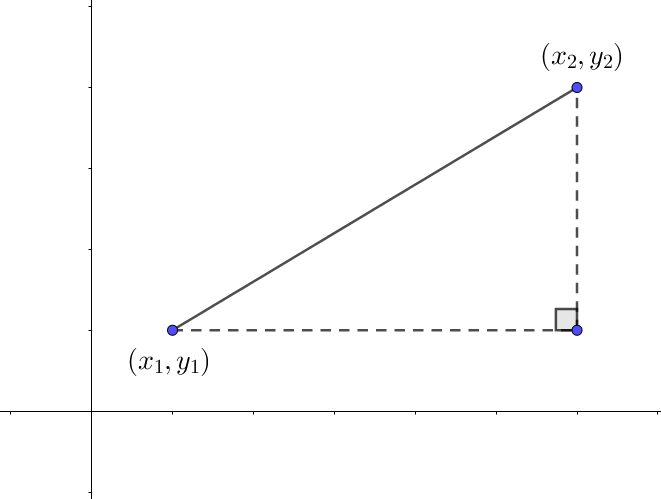
\includegraphics[width=2in]{Segment.png}

\pause

Using the drawing below, we can develop an understanding of the Distance Formula.

\pause

The length of the horizontal leg is $x_2 - x_1$, and the length of the vertical leg is $y_2 - y_1$. 

\pause

So, using the Pythagorean Theorem, we know that $$D = \sqrt{(x_2 - x_1)^2 + (y_2 - y_1)^2}$$

\end{frame}

\begin{frame}[t]{Distance and Midpoint}
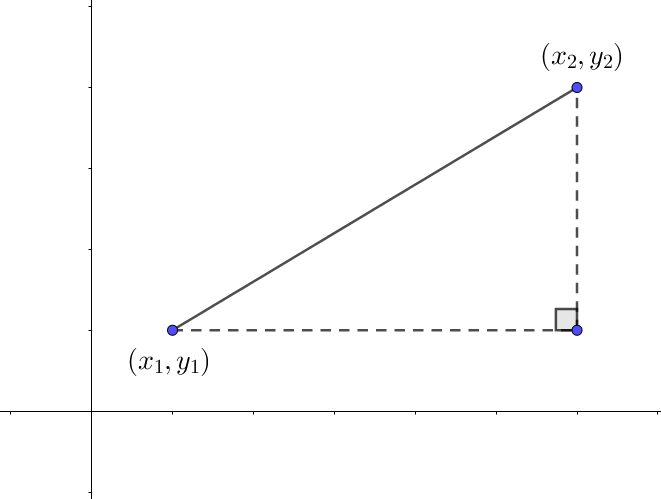
\includegraphics[width=2in]{Segment.png}

\pause

The \textit{midpoint} of a segment is the exact center.

\pause

To find it, we take the average of the $x$-coordinates and the average of the $y$-coordinates.

Midpoint = $\fp{\dfrac{x_1 + x_2}{2},\dfrac{y_1+y_2}{2}}$
\end{frame}

\begin{frame}[t]{Distance and Midpoint}
Given the points $(-2, 1)$ and $(3, 4)$, find the distance and the midpoint.
\end{frame}

\begin{frame}[t]{Applications}
Yahoo! Inc. had annual revenues of approximately \$5.0 billion in 2012 and \$4.6 billion in 2014. Without knowing any additional information, what would you estimate the 2013 revenue to have been?

\vfill \pause

An airplane flies from Naples, Italy in a straight line to Naples, Italy, which is 120 kilometers north and 150 kilometers west of Naples. How far does the plane fly?

\end{frame}

\begin{frame}[t]{Next Steps}
\begin{itemize}
\item Read 1.1 and 1.2
\item Watch Video Lesson \#4
\item Complete Assignment \#2
\end{itemize}

\vfill

Thanks for watching!
\end{frame}
\end{document}